\documentclass[amsmath, preprintnumbers, 12pt, onecolumn, pre, longbibliograpy]{revtex4-1}
\usepackage{graphicx}
\usepackage[margin = 1in]{geometry}

\usepackage{subfigure}
\usepackage{color}
\newcommand{\MW}{\mathbf W}
\newcommand{\MA}{\mathbf A}
\newcommand{\MB}{\mathbf B}
\newcommand{\MX}{\mathbf X}
\newcommand{\aff}{\mathcal A}
\newcommand{\R}{\mathcal R}
\newcommand{\vP}{\mathbf P}
\renewcommand{\Re}{{\mathrm Re}}
\renewcommand{\Im}{{\mathrm Im}}
\usepackage{physics}


\begin{document}

\thispagestyle{empty}
\noindent Dear Editors of PRE,

\vspace{1cm}

We are writing to transfer our manuscript from PRL to PRE.  
Our work shows (to the best of our knowledge for the first time) how oscillation time scales in disordered non-equilibrium Markov networks can be robustly tuned due to nonequilibrium driving. In a follow up preprint (submitted after the previous resubmission of this manuscript), we have already shown how the ideas in our paper can be extended beyond the unicyclic networks considered here (Ref.~36 of the manuscript). The referee reports from the previous rounds all recommended that the paper be accepted for publication in Physical Review. Further Referees B and D also commented positively on the broader impacts of this work. We hope that this manuscript can be considered for publication in Physical Review E. 

To further refine our manuscript and to make it better fit the usual PRE format we have made the following minor changes:
\begin{itemize}
\item Following the recommendation of some of the referees, we have reformatted the manuscript so that the derivation of the main results is now in the main text. We agree with their assessment that this ``adds to the core value" of our work, and it is now possible due to the more relaxed space constraints of PRE.
\item We moved some of the data of Fig.~3 to the manuscript to a new figure (FIg.~4) along with additional data (shown in Fig.~\ref{fig:ttriv} of this letter) that shows how our results go beyond a trivial limit raised by Referee A in the final round of reviews. We believe this strengthens our results and adds to the readability of the figures.
\item Remaining supplemental material has been moved to appendices for the reader's convenience.
\end{itemize}

Below, we provide replies to the last few questions raised by the referees and editors in the previous round. 

\section*{Point-by-point reply}

Referee comments are italicized, with our replies following in plain script.

\subsection*{Referee A}

{\it In their second resubmitted manuscript, the authors have streamlined the text to remove repetitive discussion points, added scatter plots to illustrate the accuracy of their approximative results in more detail, and clarified their use of 'disorder' in the text.}

{\it The main theoretical result of the present work is the demonstration that for higher overall affinity, the cycle coherence and period are less affected by rearrangement and random perturbations of the individual rates in a cyclic reaction network.}

{\it The main point of concern I raised in my previous report was about the biological relevance of this result as a potential explanation for the design of biological clock cycles, which have been found to use more chemical driving than minimally required for achieving a certain precision.}

{\it I argued that in a typical biological clock that gives rise to a unicyclic Markov state network, only few (~10) elementary reactions govern the kinetics, not a large number of independent random rates as assumed in the present model. To this the authors replied that "rates are affected by local fluctuations in temperature, ATP concentration and other environmental parameters. The number of parameters in the Markov state model can therefore be large even if the number of parameters in the cycle of an isolated KaiC is small". I do not find this explanation convincing. Temperature as well as ATP concentration equilibrate within at most seconds on the scale of a single cell, while the circadian cycle and even the elementary rates in KaiABC are much slower. Thus on the scale of a cell, the rate constants in the cycle are effective parameters averaged over local fluctuations. Independent random perturbations of individual MSM cycle step rates introduce artificially many parameters. This considerably weakens the biological relevance of the claim that high affinity decreases the number of relevant parameters: The demonstration that the spread of R and T values upon random perturbation of many rates decreases, does not convincingly point to a fitness advantage.}

Although the caricature in Fig.~1a of our manuscript may suggest that the only reactions in the KaiC circadian cycle are the phosphorylation and dephosphorylation of the CII domain of KaiC, leading to $\sim 10$ reactions, in fact there are many more reactions, including the binding and unbinding of KaiA, nucleotide exchange on the CI and CII domains, ATP hydrolysis at the CI domain, and binding of KaiB~\cite{Paijmans2017}. In a detailed computational model of KaiC oscillations that reproduces many experimental data (Ref.~\citenum{Paijmans2017}) there are over 30 parameters even for a single monomer. Moreover, KaiC exists as a hexamer and the reaction rates for a monomer depend on the state of the whole hexamer; the reaction rates of the hexamer depend on the state of the whole system. The networks we consider represent collective oscillations; thus, even though two edges may both represent (for instance) phosphorylation reactions at the threonine site of the KaiC CII domain, since the collective state of the system is different when each of these events occurs, they will have different rates.

The authors of Ref.~\citenum{Paijmans2017} have made their Kinetic Monte Carlo code available. In their simulation, the propensity, which corresponds to the rate of the next reaction to occur in the system, is calculated at each step. We have modified the code to output the propensities in order to see how many rates emerge in a collection of oscillating KaiC hexamers. {\bf In Fig.~\ref{fig:rates} of this letter we show a series of time traces and a histogram of the rates occurring in simulations of 10 hexamers, for which there are over 5000 propensities in a cycle.} We conclude that even without considering the effect of fluctuations, the number of parameters is generally on the order of hundreds or thousands and not on the order of 10, and it appears that it is a fair approximation to draw the rates from a distribution (we note, however, that our results do not depend on the rates being iid random variables - we simply used such rates as a case study in our numerical results). For the KaiC model, we note that {\bf much less detailed models such as the one in Ref.~\citenum{Hong2019} still contain on the order of 100 parameters.}

\begin{figure}
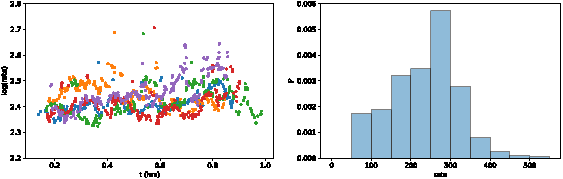
\includegraphics[width = \linewidth]{rates.pdf}
\caption{Propensities (rates) of the KaiC model in Ref.~\citenum{Paijmans2017}. On the left, we show time traces of the rates in 5 simulations of 10 KaiC hexamers using the default parameter set in the code made available by the authors of the model. All simulations were started in the same state at time 0. The total number of rates is clearly large and the time traces are different for different realizations, similar to the quenched disorder that we consider in our manuscript.  On the right, we show a histogram of all of the rates of all 5 simulations over one period, from $t = 24 - 48$ hours. For visual clarity,  in these plots we do not include a very small (less than 1\%) subset of the rates that are orders of magnitude larger than the other rates. These very fast rates contribute minimally to the time scales of oscillations.}
\label{fig:rates}
\end{figure}

{\it In sum, I think that while the paper is accessible, original and appears methodically sound, its main results do not have the broad implications that would warrant a publication in PRL. I would recommend publication in a more specialized journal. I do apologize for not providing a stronger opinion on the previous round of reports, which might have shortened the review process.}

The referee's doubt about the number of parameters in oscillators such as KaiABC appears to be the main reason that they believe our paper does not have broad enough implications.  We hope that by demonstrating that the KaiABC oscillator has a wide distribution of rates per cycle, we have convincingly argued that the behavior of models with many rates is in fact relevant to biological oscillators, and that our results can therefore have broad implications. We also note that the reason the KaiABC oscillator has many rates is that reaction rates depend on the state of the whole system. This is a general property of systems with feedback that exhibit collective oscillations~\cite{Marsland2019}, so we expect that Markov state models of these systems will generally contain many parameters.

{\it A few additional remarks that the authors might want to consider for a future version of this work:}

{\it 1. Concerning the main theoretical result: In the limit of irreversible steps, which the high-affinity case approaches, it is not surprising that the arrangement of step rates is irrelevant. This can be seen by considering the classical quantification of cycle coherence as the coefficient of variation of the stochastic period T, i.e. the completion time of one full cycle (see e.g. http://symposium.cshlp.org/content/60/793). Indeed, T is a sum of statistically independent individual step completion times; as such its distribution is independent of the step order. Although the cycle coherence definition used here is not the same, the physical content is very similar, and thus the robustness to rearrangements at high affinity is to be expected.}

Indeed, in the limit of very high affinity where all reverse reactions are suppressed, the period of the oscillator is simply expected to be $T = \sum_i 1/k_i^+$. However, {\bf we emphasize that our result work even where there is a high probability of reverse steps: with an affinity $\mathcal A_0/N = 0.5$ the average ratio of forward to reverse rates is $\exp(0.5) \approx 1.65$, and our theory still makes good approximations for $T$ and $\mathcal R$ in this regime (See Fig 2 of our Manuscript)}. Comparing with the paper by Schnitzer and Block (S and B) suggested by the referee (which we thank them for pointing out as we were not aware of it), our theory deals with cases where, unlike in Eq.~24 of S and B, \textit{all} of the reverse reaction rates $k_{-i}$ are nonzero. Our theory thus works in cases far from both known limits (the symmetric limit where all rates are equal, and the infinite affinity limit where all reverse rates can be neglected). To illustrate this, in Fig.~\ref{fig:ttriv} of this letter we reproduce the scatter plot from Fig.~3b of our manuscript where none of the rates are equal to one another, to which we have added points representing the trivial guess  $T = \sum_i 1/k_i^+$. {\bf The bounds on oscillator coherence in the literature~\cite{Barato2017, Cao2015} are saturated only in the symmetric limit, and thus are unable to give insight in to the role of energy dissipation when there is significant disorder. Our analytical theory allows us to make statements about time scales and the role of energy consumption in oscillator models with many different rates.}

\begin{figure}
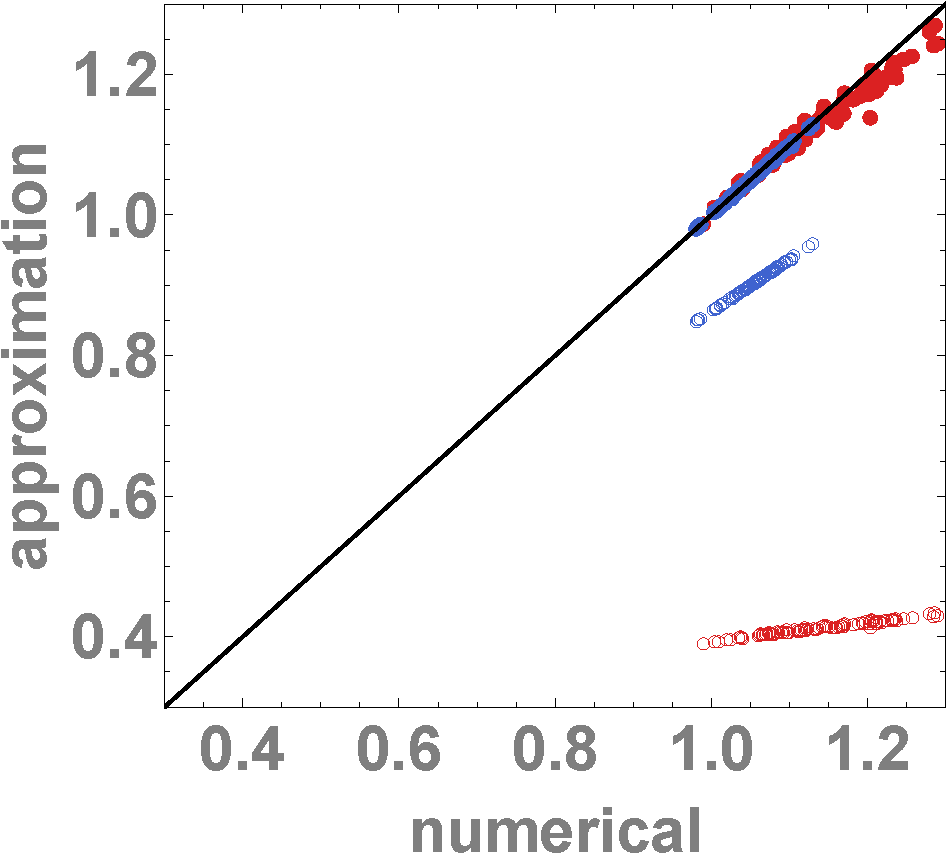
\includegraphics[width = 0.45\linewidth]{ttriv.pdf}
\caption{$T/T_0$ where $T_0$ is the period of a uniform network with all $k^+ = \exp(\mathcal A_0/N)$ and $k^- = 1$. Each point represents the period of a network with randomly generated rates as in Fig.~3b of the manuscript, calculated numerically and from an analytical approximation. Red (blue) points are for $\mathcal A_0/N = 0.5 (2)$. Filled circles are given by our theory; open circles by the approximation in the limit where reverse steps can be neglected ($T = \sum_i 1/k_i^+$). At $\mathcal A_0/N = 0.5$, where neglecting reverse steps underestimates the period by more than 50\%, our theory provides an accurate estimate. Note that in Fig.~3b of the manuscript we plotted $(T/T_0)^{-1}$; here we plot $(T/T_0)$ simply because it results in a more compact plot.}
\label{fig:ttriv}
\end{figure}

{\it 2. I find the use of the wording `fluctuations in the rates' confusing, since this evokes $temporal$ fluctuations, while the article considers frozen heterogeneity, i.e. rates that remain constant at least over $\mathcal R$ cycle periods.}

Thanks for this comment. We have replaced the term ``fluctuations" with ``disorder" and further clarified that we consider quenched disorder.

%In the manuscript, we use quenched disorder for two reasons: first, to consider the synchronization between multiple noninteracting oscillators (e.g. in different cells~\cite{Mihalcescu2004}) and second, to consider the variation in a single oscillator's properties when the rates are fluctuating over time. 
%
%With regards to the period of the oscillator we think that using quenched disorder is a good proxy for temporal fluctuations, because comparing two different realizations of quenched disorder is similar to comparing two cycles of the same oscillator where the rates are different between the first and second oscillations due to temporal fluctuations. In practice a rate may also have changed many times over the course of the period between being visited the $n$th and $n+1$th time by the system; the system does not `see' these changes so only two rates are necessary to capture the effects of the rates changing over time.
%
%As the referee says, when comparing values of $\mathcal R$, on the other hand, the rates should remain the same for at least $\mathcal R$ cycles. However, since one of our main results is that increasing affinity makes values of $\R$ more consistent between different oscillators with similarly distributed rates, we believe that all of our conclusions for $\R$ should hold if we were to perform calculation with explicit time-dependence, i.e. by using kinetic Monte Carlo simulations to simulate systems with time-varying rates.

{\it 3. One aspect of the results I did find biologically potentially interesting: The inverse scaled cycle time ($T_0/T$) decreases less strongly with increasing spread of perturbed rates for higher affinity (fig.3 lower left). Does this also mean that the raw average cycle time $<T>$ is less affected by changes in $\mathcal A_0$ for higher $\mathcal A_0$? (I don't think that's shown in fig 3. since everything is scaled by $T_0$ which is $\mathcal A_0$ dependent.) In that case one could potentially argue that across a cell population, different cells' cycle period is not as easily affected by ATP levels or temperature, which may be different from cell to cell. Temperature compensation is one of the defining features of circadian rhythms, and a contribution of high affinity to temperature compensation might be of interest.}

The raw average cycle time is not less affected by changes in $\mathcal A_0$ for higher $\mathcal A_0$ in these unicyclic models. However, in a follow-up paper, we consider how networks designed with multiple cycles can have this property~\cite{DelJunco2019b}.

\subsection*{Referee D}

{\it This is a very nice manuscript by del Junco and Vaikuntanathan addressing the robustness of biochemical cycles. I find particularly interesting the use of random matrix methods in this context. In my opinion this is a strength of the manuscript, which brings together different areas of research. I see a potential for broadening these connections.}

{\it My main concern is the degree of generality of the model and thus, of the approach. Biochemical oscillators generally require a negative feedback, see Novak and Tyson (2008), ref. [3] of the manuscript. The model described in the manuscript does not include such feedback, but rather describes a closed cycle of reactions, in line with the work of Barato and Seifert (2017). This may be alright for the KaiABC system of cyanobacteria, where there is a cycle of phosphorylation/de-phosphorylation reactions that drives the assembly/disassembly of the protein complex in vitro without feedback, see Nakajima et al. (2005). However, even this KaiABC system comprises a negative feedback in vivo, where by the way its precision is remarkably high, see Mihalcescu et al. (2004).}

{\it Now, the authors motivate the model from the fact that biochemical oscillators undergo noisy limit cycles. They propose that the N states connected in a ring may represent a projection of an oscillator's average limit cycle. Yet they give as an example ``the well-studied KaiABC oscillator of the cyanobacteria S. elongatus, each of these states would represent a vector of counts of the different phosphorylation states of a population of KaiC proteins". I think this is somewhat confusing, because in the specific case of the in vitro KaiABC oscillator there is no feedback and one can actually represent the process as a closed cycle of reactions. But in the more general case of a biochemical oscillator including negative feedback, such mapping is not possible because the model lacks a feedback step.}

{\it In summary, (i) it is not clear to me how the feedback step is contemplated in a model that consists of a closed sequence of reactions, how it would be represented as a single or several reaction steps, and (ii) I think that the specific KaiABC cycle is not a good example for the more generic interpretation that the authors propose, that the reaction steps represent points in the noisy limit cycle projection.}

We thank the referee for these positive and helpful comments. As discussed in the review article by Novak and Tyson~\cite{Novak2008}, negative feedback is a necessary condition for oscillations, and the KaiABC post-translational oscillator (i.e. in vitro) is no exception. The negative feedback takes the form of the inhibition of KaiC phosphorylation by KaiC hexamers that are already fully phosphorylated, mediated by KaiA sequestration. The in vivo oscillator contains additional negative feedback loops that increase the robustness of the clock, as the referee mentions. We clarify (and have clarified at the end of the manuscript) that the closed cycle of states is a more detailed representation of the emergent oscillations that encodes this negative feedback in the rates of hopping between different collective states of the system. Indeed, as discussed in Ref.~\cite{Marsland2019}, the requirement of negative feedback means that rates must depend on the collective state of system, implying that in the cyclic Markov models considered in our manuscript and in Ref.~\cite{Barato2017} and others, the rates {\it cannot} be uniform. This provides another motivation for our study of networks with many different rates.

Since any oscillator undergoes a limit cycle (by definition) and the Markov network is simply a stochastic, discrete representation of this limit cycle at finite copy number, we expect this representation to be generic. There is no requirement that the total number of molecules in the system remain fixed; for instance, a hop between neighboring states could represent an increment in the population of a protein due to a translation event. The only requirement is that the system proceeds through a series of collective states cyclically; it is not necessary that a given protein complex does so. Thus, a translation-transcription oscillator could also be described in this way. On the other hand, there are other limits to our representation; in particular, we do not expect most oscillators to be adequately represented by a single cycle. In ongoing work we are studying the formal mapping of KaiABC and other models of biochemical oscillators on to these Markov models.

{\it Aside from this caveat, I have to say that I do like the work very much, and as I said I think it contributes a bridge between areas that may have an impact in the future. I have gone through the calculations in the SM and they seem correct. Given the space I would recommend the inclusion of these in the manuscript, as I think these add to the core value of this work, which might make it more suited to a longer format.} 

{\it Taking things together I feel inclined to recommend this manuscript for PRL, maybe recommending the authors to briefly discuss how the model describes (or not) negative feedback.}
We thank the referee for this recommendation. 

\noindent Sincerely,

\noindent Clara del Junco

\noindent Suriyanarayanan Vaikuntanathan (Corresponding Author, Email: \href{mailto:svaikunt@uchicago.edu}{svaikunt@uchicago.edu})

%\bibliography{/Users/claradeljuncooffice/Dropbox/Papers/my-library.bib}

%merlin.mbs apsrev4-1.bst 2010-07-25 4.21a (PWD, AO, DPC) hacked
%Control: key (0)
%Control: author (8) initials jnrlst
%Control: editor formatted (1) identically to author
%Control: production of article title (-1) disabled
%Control: page (0) single
%Control: year (1) truncated
%Control: production of eprint (0) enabled
\begin{thebibliography}{7}%
\makeatletter
\providecommand \@ifxundefined [1]{%
 \@ifx{#1\undefined}
}%
\providecommand \@ifnum [1]{%
 \ifnum #1\expandafter \@firstoftwo
 \else \expandafter \@secondoftwo
 \fi
}%
\providecommand \@ifx [1]{%
 \ifx #1\expandafter \@firstoftwo
 \else \expandafter \@secondoftwo
 \fi
}%
\providecommand \natexlab [1]{#1}%
\providecommand \enquote  [1]{``#1''}%
\providecommand \bibnamefont  [1]{#1}%
\providecommand \bibfnamefont [1]{#1}%
\providecommand \citenamefont [1]{#1}%
\providecommand \href@noop [0]{\@secondoftwo}%
\providecommand \href [0]{\begingroup \@sanitize@url \@href}%
\providecommand \@href[1]{\@@startlink{#1}\@@href}%
\providecommand \@@href[1]{\endgroup#1\@@endlink}%
\providecommand \@sanitize@url [0]{\catcode `\\12\catcode `\$12\catcode
  `\&12\catcode `\#12\catcode `\^12\catcode `\_12\catcode `\%12\relax}%
\providecommand \@@startlink[1]{}%
\providecommand \@@endlink[0]{}%
\providecommand \url  [0]{\begingroup\@sanitize@url \@url }%
\providecommand \@url [1]{\endgroup\@href {#1}{\urlprefix }}%
\providecommand \urlprefix  [0]{URL }%
\providecommand \Eprint [0]{\href }%
\providecommand \doibase [0]{http://dx.doi.org/}%
\providecommand \selectlanguage [0]{\@gobble}%
\providecommand \bibinfo  [0]{\@secondoftwo}%
\providecommand \bibfield  [0]{\@secondoftwo}%
\providecommand \translation [1]{[#1]}%
\providecommand \BibitemOpen [0]{}%
\providecommand \bibitemStop [0]{}%
\providecommand \bibitemNoStop [0]{.\EOS\space}%
\providecommand \EOS [0]{\spacefactor3000\relax}%
\providecommand \BibitemShut  [1]{\csname bibitem#1\endcsname}%
\let\auto@bib@innerbib\@empty
%</preamble>
\bibitem [{\citenamefont {Paijmans}\ \emph {et~al.}(2017)\citenamefont
  {Paijmans}, \citenamefont {Lubensky},\ and\ \citenamefont {ten
  Wolde}}]{Paijmans2017}%
  \BibitemOpen
  \bibfield  {author} {\bibinfo {author} {\bibfnamefont {J.}~\bibnamefont
  {Paijmans}}, \bibinfo {author} {\bibfnamefont {D.~K.}\ \bibnamefont
  {Lubensky}}, \ and\ \bibinfo {author} {\bibfnamefont {P.~R.}\ \bibnamefont
  {ten Wolde}},\ }\href {\doibase 10.1016/J.BPJ.2017.05.048} {\bibfield
  {journal} {\bibinfo  {journal} {Biophys. J.}\ }\textbf {\bibinfo {volume}
  {113}},\ \bibinfo {pages} {157} (\bibinfo {year} {2017})}\BibitemShut
  {NoStop}%
\bibitem [{\citenamefont {Hong}\ \emph {et~al.}(2019)\citenamefont {Hong},
  \citenamefont {Lavrentovich}, \citenamefont {Chavan}, \citenamefont
  {Leypunskiy}, \citenamefont {Li}, \citenamefont {Matthews}, \citenamefont
  {LiWang}, \citenamefont {Rust},\ and\ \citenamefont {Dinner}}]{Hong2019}%
  \BibitemOpen
  \bibfield  {author} {\bibinfo {author} {\bibfnamefont {L.}~\bibnamefont
  {Hong}}, \bibinfo {author} {\bibfnamefont {D.~O.}\ \bibnamefont
  {Lavrentovich}}, \bibinfo {author} {\bibfnamefont {A.}~\bibnamefont
  {Chavan}}, \bibinfo {author} {\bibfnamefont {E.}~\bibnamefont {Leypunskiy}},
  \bibinfo {author} {\bibfnamefont {E.}~\bibnamefont {Li}}, \bibinfo {author}
  {\bibfnamefont {C.}~\bibnamefont {Matthews}}, \bibinfo {author}
  {\bibfnamefont {A.}~\bibnamefont {LiWang}}, \bibinfo {author} {\bibfnamefont
  {M.~J.}\ \bibnamefont {Rust}}, \ and\ \bibinfo {author} {\bibfnamefont
  {A.~R.}\ \bibnamefont {Dinner}},\ }\href {\doibase 10.1101/835280} {\bibfield
   {journal} {\bibinfo  {journal} {bioRxiv}\ } (\bibinfo {year} {2019}),\
  10.1101/835280},\ \Eprint
  {http://arxiv.org/abs/https://www.biorxiv.org/content/early/2019/11/08/835280.full.pdf}
  {https://www.biorxiv.org/content/early/2019/11/08/835280.full.pdf}
  \BibitemShut {NoStop}%
\bibitem [{\citenamefont {Mihalcescu}\ \emph {et~al.}(2004)\citenamefont
  {Mihalcescu}, \citenamefont {Hsing},\ and\ \citenamefont
  {Leibler}}]{Mihalcescu2004}%
  \BibitemOpen
  \bibfield  {author} {\bibinfo {author} {\bibfnamefont {I.}~\bibnamefont
  {Mihalcescu}}, \bibinfo {author} {\bibfnamefont {W.}~\bibnamefont {Hsing}}, \
  and\ \bibinfo {author} {\bibfnamefont {S.}~\bibnamefont {Leibler}},\
  }\href@noop {} {\bibfield  {journal} {\bibinfo  {journal} {Nature}\ }\textbf
  {\bibinfo {volume} {430}},\ \bibinfo {pages} {81} (\bibinfo {year}
  {2004})}\BibitemShut {NoStop}%
\bibitem [{\citenamefont {del Junco}\ and\ \citenamefont
  {Vaikuntanathan}(2019)}]{DelJunco2019b}%
  \BibitemOpen
  \bibfield  {author} {\bibinfo {author} {\bibfnamefont {C.}~\bibnamefont {del
  Junco}}\ and\ \bibinfo {author} {\bibfnamefont {S.}~\bibnamefont
  {Vaikuntanathan}},\ }\href@noop {} {\enquote {\bibinfo {title} {Robust
  oscillations in multi-cyclic models of biochemical clocks},}\ } (\bibinfo
  {year} {2019}),\ \Eprint {http://arxiv.org/abs/1909.02534} {arXiv:1909.02534
  [cond-mat.stat-mech]} \BibitemShut {NoStop}%
\bibitem [{\citenamefont {Nov{\'{a}}k}\ and\ \citenamefont
  {Tyson}(2008)}]{Novak2008}%
  \BibitemOpen
  \bibfield  {author} {\bibinfo {author} {\bibfnamefont {B.}~\bibnamefont
  {Nov{\'{a}}k}}\ and\ \bibinfo {author} {\bibfnamefont {J.~J.}\ \bibnamefont
  {Tyson}},\ }\href {\doibase 10.1038/nrm2530} {\bibfield  {journal} {\bibinfo
  {journal} {Nat. Rev. Mol. Cell Biol.}\ }\textbf {\bibinfo {volume} {9}},\
  \bibinfo {pages} {981} (\bibinfo {year} {2008})}\BibitemShut {NoStop}%
\bibitem [{\citenamefont {Marsland}\ \emph {et~al.}(2019)\citenamefont
  {Marsland}, \citenamefont {Cui},\ and\ \citenamefont
  {Horowitz}}]{Marsland2019}%
  \BibitemOpen
  \bibfield  {author} {\bibinfo {author} {\bibfnamefont {R.}~\bibnamefont
  {Marsland}}, \bibinfo {author} {\bibfnamefont {W.}~\bibnamefont {Cui}}, \
  and\ \bibinfo {author} {\bibfnamefont {J.~M.}\ \bibnamefont {Horowitz}},\
  }\href {\doibase 10.1098/rsif.2019.0098} {\bibfield  {journal} {\bibinfo
  {journal} {J. R. Soc. Interface}\ }\textbf {\bibinfo {volume} {16}},\
  \bibinfo {pages} {20190098} (\bibinfo {year} {2019})}\BibitemShut {NoStop}%
\bibitem [{\citenamefont {Barato}\ and\ \citenamefont
  {Seifert}(2017)}]{Barato2017}%
  \BibitemOpen
  \bibfield  {author} {\bibinfo {author} {\bibfnamefont {A.~C.}\ \bibnamefont
  {Barato}}\ and\ \bibinfo {author} {\bibfnamefont {U.}~\bibnamefont
  {Seifert}},\ }\href {\doibase 10.1103/PhysRevE.95.062409} {\bibfield
  {journal} {\bibinfo  {journal} {Phys. Rev. E}\ }\textbf {\bibinfo {volume}
  {95}},\ \bibinfo {pages} {062409} (\bibinfo {year} {2017})}\BibitemShut
  {NoStop}%
\bibitem [{\citenamefont {Cao}\ \emph {et~al.}(2015)\citenamefont {Cao},
  \citenamefont {Wang}, \citenamefont {Ouyang},\ and\ \citenamefont
  {Tu}}]{Cao2015}%
  \BibitemOpen
  \bibfield  {author} {\bibinfo {author} {\bibfnamefont {Y.}~\bibnamefont
  {Cao}}, \bibinfo {author} {\bibfnamefont {H.}~\bibnamefont {Wang}}, \bibinfo
  {author} {\bibfnamefont {Q.}~\bibnamefont {Ouyang}}, \ and\ \bibinfo {author}
  {\bibfnamefont {Y.}~\bibnamefont {Tu}},\ }\href {\doibase 10.1038/nphys3412}
  {\bibfield  {journal} {\bibinfo  {journal} {Nat. Phys.}\ }\textbf {\bibinfo
  {volume} {11}},\ \bibinfo {pages} {772} (\bibinfo {year} {2015})}\BibitemShut
  {NoStop}%
  \end{thebibliography}%
\end{document}